\documentclass[ngerman,]{scrartcl}
\usepackage{lmodern}
\usepackage{amssymb,amsmath}
\usepackage{ifxetex,ifluatex}
\usepackage{fixltx2e} % provides \textsubscript
\ifnum 0\ifxetex 1\fi\ifluatex 1\fi=0 % if pdftex
  \usepackage[T1]{fontenc}
  \usepackage[utf8]{inputenc}
\else % if luatex or xelatex
  \ifxetex
    \usepackage{mathspec}
  \else
    \usepackage{fontspec}
  \fi
  \defaultfontfeatures{Ligatures=TeX,Scale=MatchLowercase}
\fi
% use upquote if available, for straight quotes in verbatim environments
\IfFileExists{upquote.sty}{\usepackage{upquote}}{}
% use microtype if available
\IfFileExists{microtype.sty}{%
\usepackage[]{microtype}
\UseMicrotypeSet[protrusion]{basicmath} % disable protrusion for tt fonts
}{}
\PassOptionsToPackage{hyphens}{url} % url is loaded by hyperref
\usepackage[unicode=true]{hyperref}
\hypersetup{
            pdftitle={802.11p - Umsetzung},
            pdfauthor={Dominik Bayerl},
            pdfborder={0 0 0},
            breaklinks=true}
\urlstyle{same}  % don't use monospace font for urls
\ifnum 0\ifxetex 1\fi\ifluatex 1\fi=0 % if pdftex
  \usepackage[shorthands=off,main=ngerman]{babel}
\else
  \usepackage{polyglossia}
  \setmainlanguage[]{german}
\fi
\usepackage{longtable,booktabs}
% Fix footnotes in tables (requires footnote package)
\IfFileExists{footnote.sty}{\usepackage{footnote}\makesavenoteenv{long table}}{}
\usepackage{graphicx,grffile}
\makeatletter
\def\maxwidth{\ifdim\Gin@nat@width>\linewidth\linewidth\else\Gin@nat@width\fi}
\def\maxheight{\ifdim\Gin@nat@height>\textheight\textheight\else\Gin@nat@height\fi}
\makeatother
% Scale images if necessary, so that they will not overflow the page
% margins by default, and it is still possible to overwrite the defaults
% using explicit options in \includegraphics[width, height, ...]{}
\setkeys{Gin}{width=\maxwidth,height=\maxheight,keepaspectratio}
\IfFileExists{parskip.sty}{%
\usepackage{parskip}
}{% else
\setlength{\parindent}{0pt}
\setlength{\parskip}{6pt plus 2pt minus 1pt}
}
\setlength{\emergencystretch}{3em}  % prevent overfull lines
\providecommand{\tightlist}{%
  \setlength{\itemsep}{0pt}\setlength{\parskip}{0pt}}
\setcounter{secnumdepth}{0}
% Redefines (sub)paragraphs to behave more like sections
\ifx\paragraph\undefined\else
\let\oldparagraph\paragraph
\renewcommand{\paragraph}[1]{\oldparagraph{#1}\mbox{}}
\fi
\ifx\subparagraph\undefined\else
\let\oldsubparagraph\subparagraph
\renewcommand{\subparagraph}[1]{\oldsubparagraph{#1}\mbox{}}
\fi

% set default figure placement to htbp
\makeatletter
\def\fps@figure{htbp}
\makeatother

\usepackage{siunitx}
\usepackage{cleveref}

\title{802.11p - Umsetzung}
\author{Dominik Bayerl}
\date{}

\begin{document}
\maketitle

% pandoc-xnos: cleveref fakery
\newcommand{\plusnamesingular}{}
\newcommand{\starnamesingular}{}
\newcommand{\xrefname}[1]{\protect\renewcommand{\plusnamesingular}{#1}}
\newcommand{\Xrefname}[1]{\protect\renewcommand{\starnamesingular}{#1}}
\providecommand{\cref}{\plusnamesingular~\ref}
\providecommand{\Cref}{\starnamesingular~\ref}
\providecommand{\crefformat}[2]{}
\providecommand{\Crefformat}[2]{}

% pandoc-xnos: cleveref formatting
\crefformat{figure}{fig.~#2#1#3}
\Crefformat{figure}{Figure~#2#1#3}
\crefformat{table}{Tab.~#2#1#3}
\Crefformat{table}{Table~#2#1#3}

\section{2. Umsetzung}\label{umsetzung}

Im Rahmen des Projekts wurden die zwei grundsätzlichen Funktionen
umgesetzt, die zur Nutzung der Hardware für weitere Experimente
erforderlich sind. Dies ist einerseits die Erweiterung des
802.11-Reference-Designs auf den 802.11p-Standard und andererseits die
Implementierung einer Ethernet-Schnittstelle zum Empfang und Senden von
Daten über einen angeschlossenen Computer. Auf beide Funktionen soll im
Folgenden kurz eingegangen werden.

\subsection{2.1. WARP Reference Design für
802.11p}\label{warp-reference-design-fuxfcr-802.11p}

Auf die grundsätzliche Funktionsweise von \emph{802.11p} wurde bereits
in \textbf{TODO: Referenz 802.11p} eingegangen. Dabei wurde deutlich,
dass der Standard sehr ähnlich zum bereits implementierten
\emph{802.11a} ist (insbesondere die OFDM-Waveform) und sich vor allem
in zwei wesentlichen Merkmalen, den Channel-Frequenzen und der
Channel-Bandbreite unterscheidet. Es bietet sich daher an, die
Implementierung auf Basis des vorhandenen Frameworks vorzunehmen.

\subsubsection{2.1.1. Channel-Frequenzen}\label{channel-frequenzen}

Für das Teilnehmer-Multiplexing in WLAN-Funksystemen werden
üblicherweise Channels verwendet, d.h. es können mehrere getrennte
Funknetze dadurch unabhängig voneinander existieren, indem sie
verschiedene Channels und dadurch verschiedene Frequenzen für die
Kommunikation nutzen. Im 802.11p Standard sind acht verschiedene
Channel-Typen spezifiziert, die für unterschiedliche Aufgaben reserviert
sind. \Xrefname{Table}\Cref{tbl:channels} gibt einen Überblick über die
spezifizierten Kanäle (\emph{Draft ETSI EN 302 663 V1.2.0} 2012).

\begin{longtable}[]{@{}lllll@{}}
\caption{802.11p Channels. \label{tbl:channels}}\tabularnewline
\toprule
\begin{minipage}[b]{0.08\columnwidth}\raggedright\strut
Channel Type\strut
\end{minipage} & \begin{minipage}[b]{0.30\columnwidth}\raggedright\strut
Center frequency\strut
\end{minipage} & \begin{minipage}[b]{0.16\columnwidth}\raggedright\strut
IEEE 802.11 channel number\strut
\end{minipage} & \begin{minipage}[b]{0.14\columnwidth}\raggedright\strut
Channel spacing\strut
\end{minipage} & \begin{minipage}[b]{0.18\columnwidth}\raggedright\strut
Default data rate\strut
\end{minipage}\tabularnewline
\midrule
\endfirsthead
\toprule
\begin{minipage}[b]{0.08\columnwidth}\raggedright\strut
Channel Type\strut
\end{minipage} & \begin{minipage}[b]{0.30\columnwidth}\raggedright\strut
Center frequency\strut
\end{minipage} & \begin{minipage}[b]{0.16\columnwidth}\raggedright\strut
IEEE 802.11 channel number\strut
\end{minipage} & \begin{minipage}[b]{0.14\columnwidth}\raggedright\strut
Channel spacing\strut
\end{minipage} & \begin{minipage}[b]{0.18\columnwidth}\raggedright\strut
Default data rate\strut
\end{minipage}\tabularnewline
\midrule
\endhead
\begin{minipage}[t]{0.08\columnwidth}\raggedright\strut
G5-CCH\strut
\end{minipage} & \begin{minipage}[t]{0.30\columnwidth}\raggedright\strut
\(\SI{5900}{\mega\hertz}\)\strut
\end{minipage} & \begin{minipage}[t]{0.16\columnwidth}\raggedright\strut
180\strut
\end{minipage} & \begin{minipage}[t]{0.14\columnwidth}\raggedright\strut
\(\SI{10}{\mega\hertz}\)\strut
\end{minipage} & \begin{minipage}[t]{0.18\columnwidth}\raggedright\strut
\(\SI{6}{Mbps}\)\strut
\end{minipage}\tabularnewline
\begin{minipage}[t]{0.08\columnwidth}\raggedright\strut
G5-SCH2\strut
\end{minipage} & \begin{minipage}[t]{0.30\columnwidth}\raggedright\strut
\(\SI{5890}{\mega\hertz}\)\strut
\end{minipage} & \begin{minipage}[t]{0.16\columnwidth}\raggedright\strut
178\strut
\end{minipage} & \begin{minipage}[t]{0.14\columnwidth}\raggedright\strut
\(\SI{10}{\mega\hertz}\)\strut
\end{minipage} & \begin{minipage}[t]{0.18\columnwidth}\raggedright\strut
\(\SI{12}{Mbps}\)\strut
\end{minipage}\tabularnewline
\begin{minipage}[t]{0.08\columnwidth}\raggedright\strut
G5-SCH1\strut
\end{minipage} & \begin{minipage}[t]{0.30\columnwidth}\raggedright\strut
\(\SI{5880}{\mega\hertz}\)\strut
\end{minipage} & \begin{minipage}[t]{0.16\columnwidth}\raggedright\strut
176\strut
\end{minipage} & \begin{minipage}[t]{0.14\columnwidth}\raggedright\strut
\(\SI{10}{\mega\hertz}\)\strut
\end{minipage} & \begin{minipage}[t]{0.18\columnwidth}\raggedright\strut
\(\SI{6}{Mbps}\)\strut
\end{minipage}\tabularnewline
\begin{minipage}[t]{0.08\columnwidth}\raggedright\strut
G5-SCH3\strut
\end{minipage} & \begin{minipage}[t]{0.30\columnwidth}\raggedright\strut
\(\SI{5870}{\mega\hertz}\)\strut
\end{minipage} & \begin{minipage}[t]{0.16\columnwidth}\raggedright\strut
174\strut
\end{minipage} & \begin{minipage}[t]{0.14\columnwidth}\raggedright\strut
\(\SI{10}{\mega\hertz}\)\strut
\end{minipage} & \begin{minipage}[t]{0.18\columnwidth}\raggedright\strut
\(\SI{6}{Mbps}\)\strut
\end{minipage}\tabularnewline
\begin{minipage}[t]{0.08\columnwidth}\raggedright\strut
G5-SCH4\strut
\end{minipage} & \begin{minipage}[t]{0.30\columnwidth}\raggedright\strut
\(\SI{5860}{\mega\hertz}\)\strut
\end{minipage} & \begin{minipage}[t]{0.16\columnwidth}\raggedright\strut
172\strut
\end{minipage} & \begin{minipage}[t]{0.14\columnwidth}\raggedright\strut
\(\SI{10}{\mega\hertz}\)\strut
\end{minipage} & \begin{minipage}[t]{0.18\columnwidth}\raggedright\strut
\(\SI{6}{Mbps}\)\strut
\end{minipage}\tabularnewline
\begin{minipage}[t]{0.08\columnwidth}\raggedright\strut
G5-SCH5\strut
\end{minipage} & \begin{minipage}[t]{0.30\columnwidth}\raggedright\strut
\(\SI{5850}{\mega\hertz}\)\strut
\end{minipage} & \begin{minipage}[t]{0.16\columnwidth}\raggedright\strut
182\strut
\end{minipage} & \begin{minipage}[t]{0.14\columnwidth}\raggedright\strut
\(\SI{10}{\mega\hertz}\)\strut
\end{minipage} & \begin{minipage}[t]{0.18\columnwidth}\raggedright\strut
\(\SI{6}{Mbps}\)\strut
\end{minipage}\tabularnewline
\begin{minipage}[t]{0.08\columnwidth}\raggedright\strut
G5-SCH6\strut
\end{minipage} & \begin{minipage}[t]{0.30\columnwidth}\raggedright\strut
\(\SI{5910}{\mega\hertz}\)\strut
\end{minipage} & \begin{minipage}[t]{0.16\columnwidth}\raggedright\strut
184\strut
\end{minipage} & \begin{minipage}[t]{0.14\columnwidth}\raggedright\strut
\(\SI{10}{\mega\hertz}\)\strut
\end{minipage} & \begin{minipage}[t]{0.18\columnwidth}\raggedright\strut
\(\SI{6}{Mbps}\)\strut
\end{minipage}\tabularnewline
\begin{minipage}[t]{0.08\columnwidth}\raggedright\strut
G5-SCH7\strut
\end{minipage} & \begin{minipage}[t]{0.30\columnwidth}\raggedright\strut
nach IEEE 802.11, \(\SIrange{5470}{5725}{\mega\hertz}\)\strut
\end{minipage} & \begin{minipage}[t]{0.16\columnwidth}\raggedright\strut
94 bis 145\strut
\end{minipage} & \begin{minipage}[t]{0.14\columnwidth}\raggedright\strut
verschiedene\strut
\end{minipage} & \begin{minipage}[t]{0.18\columnwidth}\raggedright\strut
abhängig von der Bandbreite\strut
\end{minipage}\tabularnewline
\bottomrule
\end{longtable}

Es wird deutlich, dass eine Erweiterung des verfügbaren Frequenzbandes
von 802.11a (\(\SIrange{5180}{5825}{\mega\hertz}\)) auf 802.11p
(\(\SIrange{5850}{5925}{\mega\hertz}\)) notwendig ist.

Die RF-Frequenz wird auf dem Mango WARPv3 Board durch den RF-Transceiver
MAX2829 (siehe \textbf{TODO: Referenz Hardware}) erzeugt. Dieser kann
via SPI durch die Low-CPU des FPGAs konfiguriert werden
(„max2828/max2829 single-/dual-band 802.11a/b/g world-band transceiver``
2004). Zur Einstellung der Center-Frequenz des Transceivers sind dabei
insbesondere die Register \emph{Band Select and PLL},
\emph{Integer-Divider Ratio} und \emph{Fractional-Divider Ratio}
wichtig. Über das \emph{Band Select} Register wird das Frequenzband
(\(\SI{5}{\giga\hertz}\)) ausgewählt und durch den Vorteiler (engl.
Divider) wird die Grundfrequenz des Oszillators durch einen rationalen
Teiler (Ganzzahl und Fraktion) auf den gewünschten Wert abgeleitet. Zur
Anpassung der verfügbaren Frequenzen ist daher eine Änderung der
möglichen Register-Werte des RF-Transceivers notwendig.

Im WARP Reference Design erfolgt die Konfiguration des Transceivers
durch den radio\_controller IP Core. Änderungen der Konfiguration
erfolgen also am elegantesten im Treiber des Peripherals. Konkret
bedeutet dies, dass in der Datei \texttt{edk/pcores/radio\_controller.c}
Änderungen für drei Lookup-Tables
\texttt{rc\_tuningParams\_5GHz\_freqs},
\texttt{rc\_tuningParams\_5GHz\_reg3} und
\texttt{rc\_tuningParams\_5GHz\_reg4} notwendig sind, nämlich müssen die
Register-Werte für die hinzugefügten Channels hinterlegt werden. Die
Berechnung der Werte kann händisch nach („max2828/max2829
single-/dual-band 802.11a/b/g world-band transceiver`` 2004) oder durch
das beiligende Python-Skript erfolgen.

Anschließend müssen die zusätzlichen Kanäle zur Verwendung
``freigeschalten'' werden. Dies erfolgt in der Software der Low-CPU.

\subsubsection{2.1.2. Channel Bandbreite}\label{channel-bandbreite}

Die verwendete Bandbreite des Kanals hängt direkt von der gewählten
Sampling-Rate des verwendeten ADC/DAC-Wandlers AD9963 ab. Dieser ist
ebenfalls über die SPI-Schnittstelle durch die Low-CPU konfigurierbar,
die Implementierung erfolgt über den w3\_ad\_controller Core.

Für 802.11p werden vorrangig Kanäle der Bandbreite
\(\SI{10}{\mega\hertz}\) verwendet. Diese Bandbreite ist bereits im
802.11 Reference Design implementiert, muss jedoch in der Software der
Low-CPU durch einen Aufruf der Funktion \texttt{set\_phy\_samp\_rate()}
aktiviert werden. Der \(\SI{10}{\mega\hertz}\)-Modus wird dabei durch
die Konstante \texttt{PHY\_10M} ausgewählt.

Im 802.11p Reference Design wird ist dies im
\emph{wlan\_mac\_low\_11p}-Projekt implementiert.

\subsection{2.2. Ethernet-Schnittstelle}\label{ethernet-schnittstelle}

Für das Projekt wurde beschlossen, dass die Umsetzung von Funktionalität
möglichst auf einem normalen Computer erfolgen soll. Die Gründe dafür
sind, dass dort bereits eine Vielzahl von spezialisierten Tools (u.a.
Wireshark und PCAP) vorhanden sind, deren Implementierung den Rahmen des
Projekts bei weitem sprengen würde. Zusätzlich ermöglicht wird es
dadurch einfacher ermöglicht, Fehler in der Software zu debuggen und
3rd-party Komponenten (wie beispielsweise MATLAB) anzubinden.

Die Realisierung dieser Design-Ziele erfolgt durch die Instrumentierung
des WARP v3 Board über eome Ethernet-Schnittstelle. Darüber können
sowohl Daten des WLAN-Kanals empfangen und an einen Computer
weitergeleitet, als auch Daten von einem normalen Rechner als 802.11p
Frames gesendet werden.

\subsubsection{2.2.1. Hardware}\label{hardware}

Das WARPv3 Board besitzt zwei \(\SI{1}{Gbps}\)-Ethernet-Interfaces.
Dabei ist Interface \textbf{B} durch das Reference-Design reserviert, um
darüber Experimente steuern zu können(Mango Communications 2017). Die
Schnittstelle zur Datenübertragung wurde deshalb auf Interface
\textbf{A} realisiert. Diese kann über ein normales RJ45 Ethernet-Kabel
mit einem beliebigen Rechner verbunden werden.

\subsubsection{2.2.2. RFtap}\label{rftap}

Die Übertragung der WLAN-Frames über eine Ethernet-Schnittstelle ist nur
möglich, wenn diese vorher in ein entsprechendes Transport-Protokoll
verpackt werden. Dies ist dem Umstand geschuldet, dass 802.11-Frames
keine gültigen Ethernet(-II)-Frames sind und umgekehrt. Würde das
WARP-Board die empfangenen 802.11 Frames vollständig identisch auf die
Ethernet-Schnittstelle übertragen, werden die Frames von der
Netzwerkkarte des angeschlossenen Rechners verworfen und erreichen
dessen Betriebssystem bzw. Anwendungen erst gar nicht.

Es wurden zwei verschiedene Protokolle zur Übertragung von 802.11 Frames
über die Ethernet-Schnittstelle evaluiert: - radiotap, das spezialisiert
ist auf ``{[}\ldots{}{]} 802.11 frame injection and
reception''(„radiotap``, o.~J.) - RFtap, ein Protokoll ``{[}\ldots{}{]}
designed to provide Radio Frequency (RF) metadata about
packets''(„rftap``, o.~J.)

Für beide Protokolle existiert eine gute Unterstützung in bestehenden
Netzwerk-Analyse Tools wie Wireshark. Im Rahmen des Projekts wurde das
\emph{RFtap} Protokoll in die High-CPU Software implementiert. Die
Gründe dafür sind die einfachere Implementierung gegenüber radiotap und
die erweiterte Funktionalität. Da ein RFtap-Frame verschiedenste
Payload-Pakete verpacken kann, ist es unter anderem auch möglich, damit
radiotap-Frames zu übertragen. RFtap kann folglich als Obermenge von
radiotap angesehen werden. Zusätzlich ist es mit RFtap Möglich, die
empfangenen Pakete um weitere Informationen (insbesondere physikalische
Parameter) zu annotieren. \xrefname{fig.}\cref{fig:rftap} zeigt
schematisch den Aufbau eines RFtap-Frames.

\begin{figure}
\centering
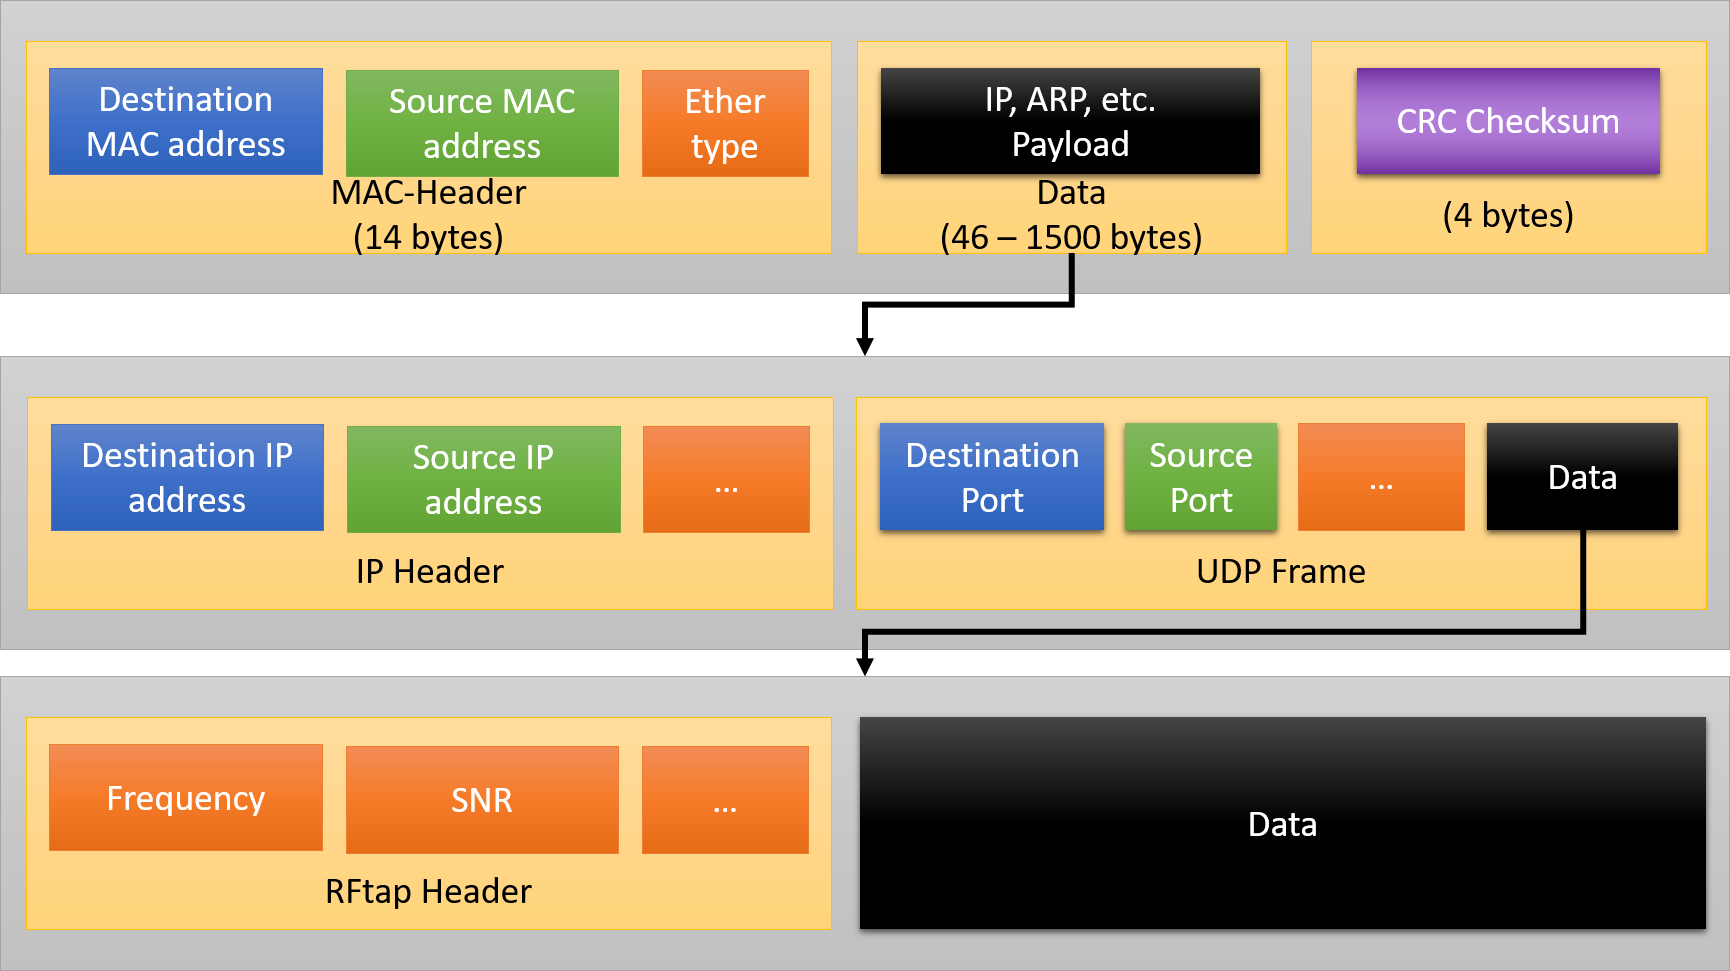
\includegraphics{rftap.png}
\caption{RFtap Frame Aufbau.\label{fig:rftap}}
\end{figure}

Für die direkte Verbindung zwischen dem WARPv3 Board und einem Computer
sind die verwendeten MAC- und IP-Adressen unkritisch, da auf den
Interfaces in diesem Fall keine Filterung stattfindet. In der
derzeitigen Implementierung sind die Felder daher leer (Wert 0). Für
künftige Projekte wäre es denkbar, diese Informationen sinnvoll zu
befüllen. Dies ermöglicht beispielsweise ein Routing von RFtap-Frames
über gewöhnliche, kommerzielle Netzwerk-Hardware.

In Wireshark sind RFtap-Dissectors für UDP-Frames auf Destination-Port
\textbf{52001} implementiert. Erkannt werden die Frames durch die Magic
Numbers \texttt{0x52\ 0x46\ 0x74\ 0x61} (ascii: RFta) zu Beginn des
Frames. Es folgt die Länge (unsigned integer, 2 Byte) des RFtap-Headers
(ohne Datenteil!) in 32-bit Words und ein Flags-Bitfield (2 Byte), das
die nachfolgenden Header-Flags spezifiziert(„specifications``, o.~J.).
Dabei können (aufgrund des Längenfelds) beliebige zusätzliche Felder an
das Ende des Headers angefügt werden, die dann jedoch nicht durch einen
Dissector abgedeckt werden können. Der RFtap-Frame endet mit dem
RF-Payload. Besonders interessant ist die Angabe des DLT-Felds, da
dadurch der Typ der Nutzdaten spezifiziert wird. Bei korrekter Angabe
nutzt Wireshark dann automatisch den richtigen Dissector um die Payload
zu analysieren (beispielsweise LINKTYPE\_IEEE802\_11, IEEE 802.11
wireless LAN Frame („link-layer header types \textbar{} tcpdump/libpcap
public repository`` 2017)).

Das Senden von Frames von einem Rechner erfolgt analog, in umgekehrter
Reihenfolge.

\emph{{[}FPGA{]}: Field Programmable Gate Array }{[}SPI{]}: Serial
Peripheral Interface \emph{{[}RF{]}: Radio Frequency }{[}ADC{]}: Analog
Digital Converter \emph{{[}DAC{]}: Digital Analog Converter }{[}DLT{]}:
Data Link Type

\hypertarget{refs}{}
\hypertarget{ref-etsi}{}
\emph{Draft ETSI EN 302 663 V1.2.0}. 2012. ETSI.

\hypertarget{ref-tcpdump}{}
„link-layer header types \textbar{} tcpdump/libpcap public repository``.
2017. \emph{tcpdump.org}. \url{http://www.tcpdump.org/linktypes.html}.

\hypertarget{ref-warp-exp}{}
Mango Communications, Inc. 2017. „Mango 802.11 Reference Design
Experiments Framework Documentation``.
\url{https://warpproject.org/docs/mango-wlan-exp/}.

\hypertarget{ref-max2829}{}
„max2828/max2829 single-/dual-band 802.11a/b/g world-band transceiver``.
2004. \emph{datasheets.maximintegrated.com}.
\url{https://datasheets.maximintegrated.com/en/ds/MAX2828-MAX2829.pdf}.

\hypertarget{ref-radiotap}{}
„radiotap``. o.~J. \emph{radiotap.org}. \url{http://www.radiotap.org/}.

\hypertarget{ref-rftap}{}
„rftap``. o.~J. \emph{rftap.github.io}. \url{https://rftap.github.io/}.

\hypertarget{ref-rftap-specifications}{}
„specifications``. o.~J. \emph{rftap.github.io}.
\url{https://rftap.github.io/specifications/}.

\end{document}
